\section{Ordem de Execução}
\label{sec:order-of-execution}

Quando discutíamos canais de áudio na seção \ref{sec:audiobus}, nós mencionamos a importância da ordem de execução. O código abaixo é uma versão expandida do exemplo de ruído filtrado daquela seção. Vamos agora explicar o conceito básico de ordem de execução, e demonstrar o por quê da sua importância.

\begin{lstlisting}[style=SuperCollider-IDE, basicstyle=\scttfamily\footnotesize]
// Criar um canal de áudio
~fxBus = Bus.audio(s, 1);
~masterBus = Bus.audio(s, 1);
// Criar SynthDefs
(
SynthDef("noise", {Out.ar(~fxBus, WhiteNoise.ar(0.5))}).add;
SynthDef("filter", {Out.ar(~masterBus, BPF.ar(in: In.ar(~fxBus), freq: MouseY.kr(1000, 5000), rq: 0.1))}).add;
SynthDef("masterOut", {arg amp = 1; Out.ar(0, In.ar(~masterBus) * Lag.kr(amp, 1))}).add;
)
// Abrir a janela Node Tree:
s.plotTree;
// Tocar os synths (observe a Node Tree)
m = Synth("masterOut");
f = Synth("filter");
n = Synth("noise");
// Volume master
m.set(\amp, 0.1);
\end{lstlisting}

Primeiro, dois canais de áudio são criados nas variáveis \texttt{$\sim$fxbus} e \texttt{$\sim$masterBus}.

Depois, três \texttt{SynthDef}s são criadas:

\begin{itemize}
\item \texttt{"noise"} é uma fonte de ruído que envia ruído branco para o canal de efeitos;
\item \texttt{"filter"} é um filtro passa-banda que toma como entrada o canal de efeitos, e envia o som processado para o canal master;
\item \texttt{"masterOut"} pega o sinal do canal master, aplica um controle de volume simples, e envia o som final (com volume ajustado) para os alto-falantes.
\end{itemize}

Observe a janela Node Tree conforme você roda os synths em ordem.

\begin{figure}[h]
\centerline{
	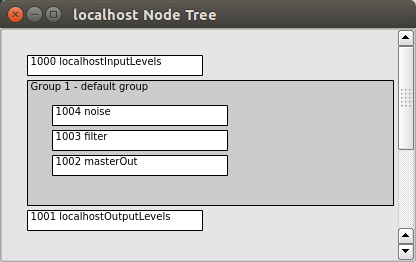
\includegraphics[scale=0.5]{fig-node-tree.png}}
\caption{A janela Node Tree}
\label{fig:node-tree}
\end{figure}

Os nós de Synth na janela Node Tree são calculados \emph{de cima pra baixo}. Os synths mais recentes são adicionados no topo da pilha. Na figura \ref{fig:node-tree}, você pode ver que \texttt{"noise"} está no topo, \texttt{"filter"} vem em segundo, e \texttt{"masterOut"} aparece por último. Esta é a ordem correta que nós queremos para este exemplo: lendo de cima para baixo, o ruído branco passa para o filtro, e o resultado do filtro passa para o canal master. Tente agora rodar o exemplo de novo, mas de trás pra frente (ou seja, rode as linhas na ordem \texttt{n}, \texttt{f}, and \texttt{m}. Você não vai ouvir nada, porque os sinais estão sendo calculados na ordem errada.

Executar as linhas certas na ordem correta é um método adequado em muitos casos, mas pode ser que isso fique um pouco complicado conforme o seu código vá ficando mais complexo. Para simplificar a tarefa, o SuperCollider permite que você defina explicitamente onde colocar os synths na janela Node Tree. Para tanto, usamos os argumentos \texttt{target} e \texttt{addAction}.

\begin{lstlisting}[style=SuperCollider-IDE, basicstyle=\scttfamily\footnotesize]
n = Synth("noise", addAction: 'addToHead');
m = Synth("masterOut", addAction: 'addToTail');
f = Synth("filter", target: n, addAction: 'addAfter');
\end{lstlisting}

Agora, não importa em que ordem você rodar as linhas acima, você pode ter certeza que os nós de cada synth vão ser colocados no lugar certo. O synth \texttt{"noise"} está sendo explicitamente adicionado na cabeça (topo) da janela Node Tree; o \texttt{"masterOut"} é adicionado na cauda (embaixo de todos os outros); e o \texttt{filter} é explicitamente adicionado logo depois do \texttt{n} (o synth de ruído).

\subsection{Grupos}

Conforme você começar a usar um monte de synths---alguns como fontes sonoras, outros para processamento, efeitos, seja lá o que você precisar---, pode ser uma boa ideia organizá-los em grupos. Aqui está um exemplo simples:

\begin{lstlisting}[style=SuperCollider-IDE, basicstyle=\scttfamily\footnotesize]
// Vá olhando tudo o que acontece na janela NodeTree
s.plotTree;

// Crie alguns canais de áudio
~reverbBus = Bus.audio(s, 2);
~masterBus = Bus.audio(s, 2);

// Defina os grupos
(
~sources = Group.new;
~effects = Group.new(~sources, \addAfter);
~master = Group.new(~effects, \addAfter);
)

// Rode todos os synths de uma vez
(
// Uma fonte de som qualquer
{
  Out.ar(~reverbBus, SinOsc.ar([800, 890])*LFPulse.ar(2)*0.1)
}.play(target: ~sources);

// Uma outra fonte sonora qualquer
{
  Out.ar(~reverbBus, WhiteNoise.ar(LFPulse.ar(2, 1/2, width: 0.05)*0.1))
}.play(target: ~sources);

// Uma pitada de reverb
{
  Out.ar(~masterBus, FreeVerb.ar(In.ar(~reverbBus, 2), mix: 0.5, room: 0.9))
}.play(target: ~effects);

// Um controle de volume com o mouse só porque é legal
{
  Out.ar(0, In.ar(~masterBus, 2) * MouseY.kr(0, 1))
}.play(target: ~master);
)
\end{lstlisting}

Para mais informações sobre ordem de execução, consulte os arquivos de ajuda ``Synth'', ``Order of Execution'' e ``Group.''
